\documentclass[11pt,a4paper]{article}

\usepackage[utf8]{inputenc}
\usepackage[T1]{fontenc}
\usepackage{lmodern}
\usepackage[margin=2.2cm]{geometry}
\usepackage{amsmath,amssymb}
\usepackage{graphicx}
\usepackage{booktabs}
\usepackage{siunitx}
\usepackage{caption}
\usepackage{subcaption}
\usepackage{float}
\usepackage{xcolor}
\usepackage{enumitem}
\usepackage{tikz}
\usepackage[colorlinks=true,linkcolor=blue!50!black,citecolor=blue!50!black,urlcolor=blue!50!black]{hyperref}

\sisetup{detect-all}
\setlength{\emergencystretch}{2em}
\setlist{nosep,leftmargin=*}
\captionsetup{font=small,labelfont=bf}
\newcommand{\Hs}{H_{m0}}
\newcommand{\Tm}{T_{m02}}
\newcommand{\question}[1]{\par\smallskip\noindent\colorbox{blue!6}{\parbox{\dimexpr\linewidth-2\fboxsep}{\textbf{Q:} \emph{#1}}}\par\smallskip}

% Logo in the upper-right corner of the first page.
% Upload your logo to the figures/ folder as figures/logo.jpg (or change the file name below).
\newcommand{\logo}{%
  \begin{tikzpicture}[remember picture,overlay]
    \node[anchor=north east,inner sep=0pt] at ([xshift=-1.5cm,yshift=-1.2cm]current page.north east)
      {\IfFileExists{figures/logo.jpg}%
        {\includegraphics[height=2cm]{figures/logo.jpg}}%
        {\fbox{\parbox[c][1.6cm][c]{3cm}{\centering\small LOGO}}}};
  \end{tikzpicture}}

\title{\logo\textbf{Offshore Wind Turbine Project -- Report I}\\[4pt]
\large Part I.A: Wave dynamics -- mean wave conditions and seasonal variability\\
at a candidate floating wind site off south-west Brittany}
\author{Jean Derin Bourdon\\ \small Sea States, Wave Propagation and Ocean Wave Energy (SSWPOWE) -- ENPC}
\date{23 October 2026}

\begin{document}

\maketitle

\begin{abstract}
\noindent
A 30-year (1996--2025) 3-hourly wave hindcast from the Copernicus Marine Service global wave reanalysis is analysed at a candidate offshore wind site located $\approx$\SI{50}{km} west of the Pointe du Raz (Brittany, France), in \SI{68.5}{m} of water.
The mean sea state is $\overline{\Hs}=\SI{2.42}{m}$, $\overline{\Tm}=\SI{6.48}{s}$, coming from \SI{284}{\degree} (WNW).
No statistically significant trend is found in wave height, period or direction over the 30 years; interannual variability (e.g.\ the 2013/14 winter) dominates.
The most frequent sea state is $\Hs\approx\SI{1.6}{m}$, $\Tm\approx\SI{4.75}{s}$. Waves come from the W--WNW sector \SI{82}{\percent} of the time and are deep-water waves \SI{95}{\percent} of the time (based on $\Tm$); most are weakly non-linear.
A strong seasonal cycle is observed: winter $\Hs$ is about twice the summer value.
\end{abstract}


%====================================================================
\section{Introduction and site description}
%====================================================================

The aim of the project is to design a floating offshore wind turbine (OWT) and its anchoring system.
This report covers Part I.A: it characterises the mean wave conditions at the selected site and their seasonal and interannual variability, answering the three questions of the assignment (Sections~\ref{sec:q1}--\ref{sec:q3}). The extreme wave conditions (Part I.B) will be treated separately.
These results will be used as boundary conditions for the wave propagation modelling (Part II) and the wave--structure interaction analysis (Part III).

\paragraph{Site selection.}
The site is located in the Atlantic approaches to Brittany, south-west of the Iroise Sea (Table~\ref{tab:site}).
It was chosen using the criteria introduced in class:
\begin{itemize}
  \item \textbf{Wind resource.} The Global Wind Atlas gives a mean wind speed of \SI{9.05}{m/s} at \SI{100}{m} hub height (power density \SI{789}{W/m^2}; Fig.~\ref{fig:site}a). This is above the \SI{8.5}{m/s} ``safe investment'' threshold. The wind rose is dominated by the SW--W sectors.
  \item \textbf{Water depth.} The EMODnet bathymetry gives a mean depth of \SI{68.5}{m} at the site. This is above the $\approx$\SI{60}{m} depth beyond which floating foundations become more economical than bottom-fixed ones \cite{windeurope2017}.
  \item \textbf{Distance to shore.} About \SI{50}{km} from Île de Sein and the Pointe du Raz. This is close enough for grid connection and far enough to limit visual impact and conflicts with coastal activities.
\end{itemize}
The seabed in this area deepens gently towards the west. Nearby points span roughly \SIrange{68}{87}{m} (Fig.~\ref{fig:site}b), so the exact depth of the turbine location should be confirmed with a local bathymetric survey.

\begin{table}[H]
\centering\small
\caption{Site characteristics and data sources.}
\label{tab:site}
\begin{tabular}{lp{0.5\linewidth}}
\toprule
Site coordinates & \SI{47.969}{\degree N}, \SI{5.494}{\degree W} \\
Nearest wave-model grid point & \SI{48.0}{\degree N}, \SI{5.4}{\degree W} ($\approx$\SI{8}{km} from the site) \\
Mean water depth $h$ (EMODnet) & \SI{68.5}{m} \\
Mean wind speed at \SI{100}{m} (Global Wind Atlas) & \SI{9.05}{m/s} \\
Distance to the coast & $\approx$\SI{50}{km} (Île de Sein / Pointe du Raz) \\
Wave data & CMEMS global wave reanalysis (MFWAM, \SI{0.2}{\degree}, 3-hourly) \cite{cmems} \\
Period & 01/01/1996 -- 31/12/2025 (30 years, \num{87664} sea states, no gaps) \\
\bottomrule
\end{tabular}
\end{table}

\begin{figure}[H]
\centering
\begin{subfigure}[b]{0.56\linewidth}\centering
  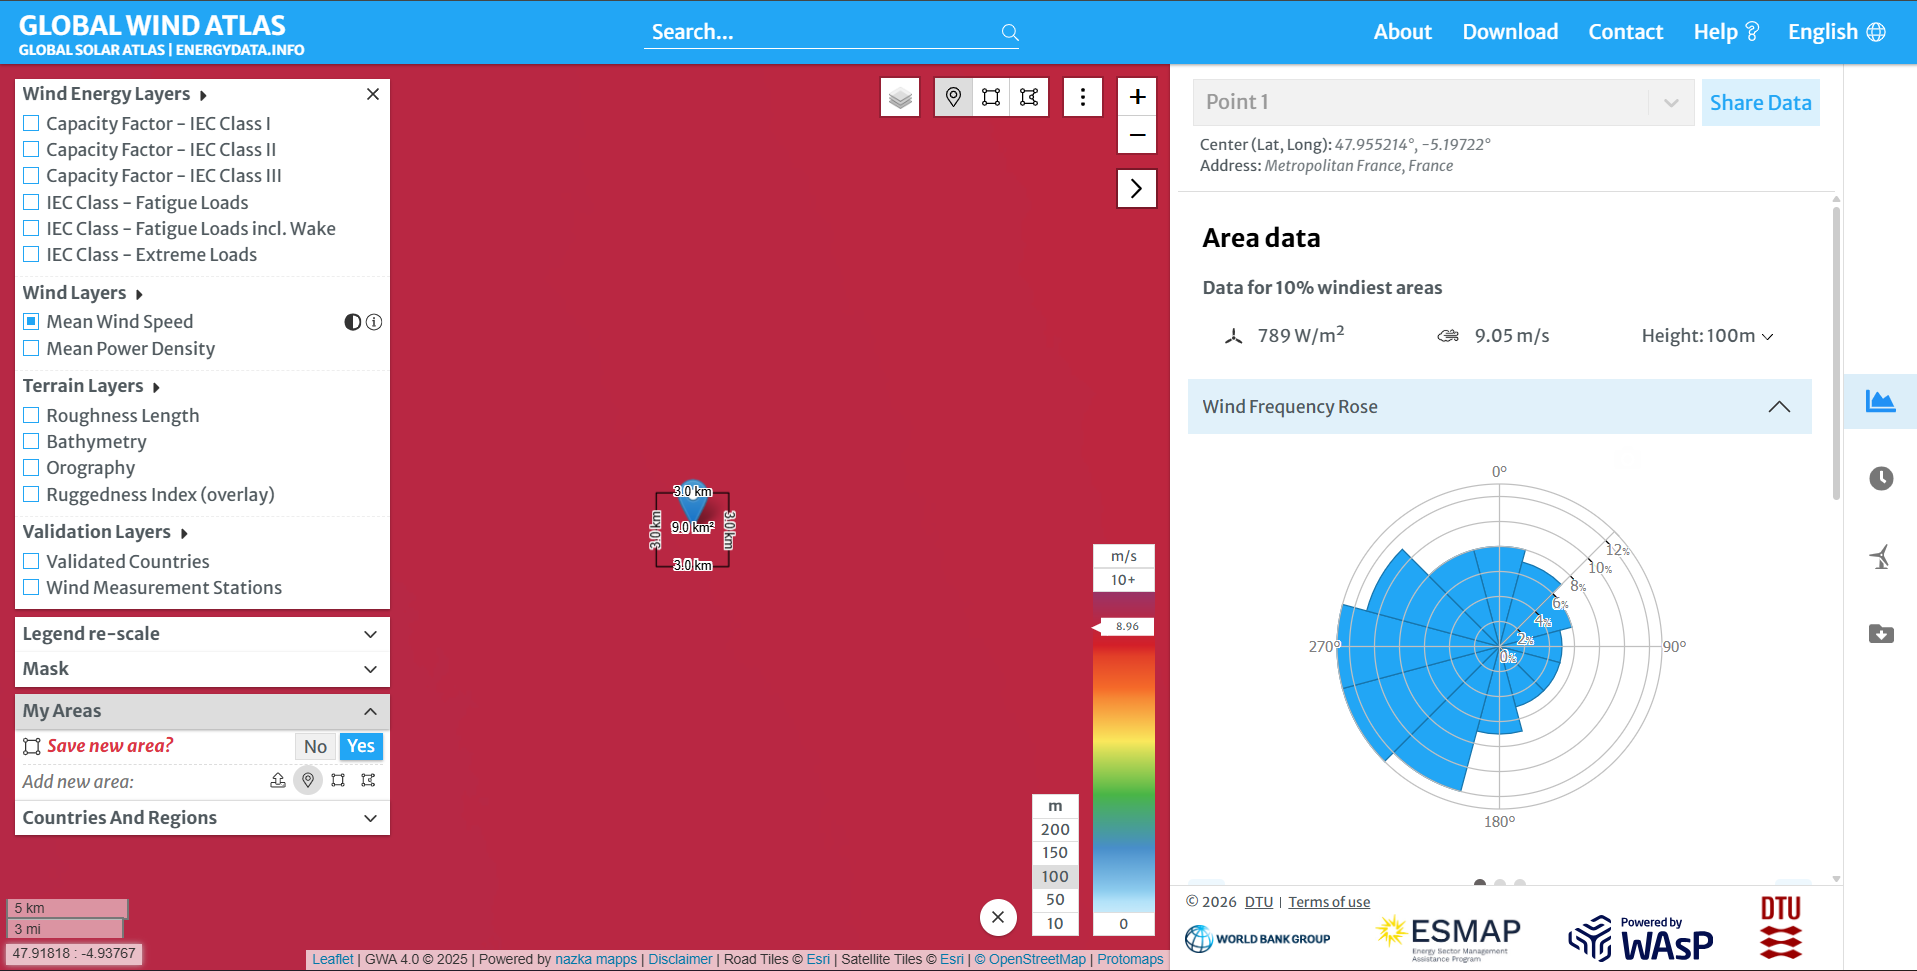
\includegraphics[width=\linewidth]{figures/global_wind_atlas.png}
  \caption{Global Wind Atlas: mean wind speed and wind rose at \SI{100}{m}.}
\end{subfigure}\hfill
\begin{subfigure}[b]{0.42\linewidth}\centering
  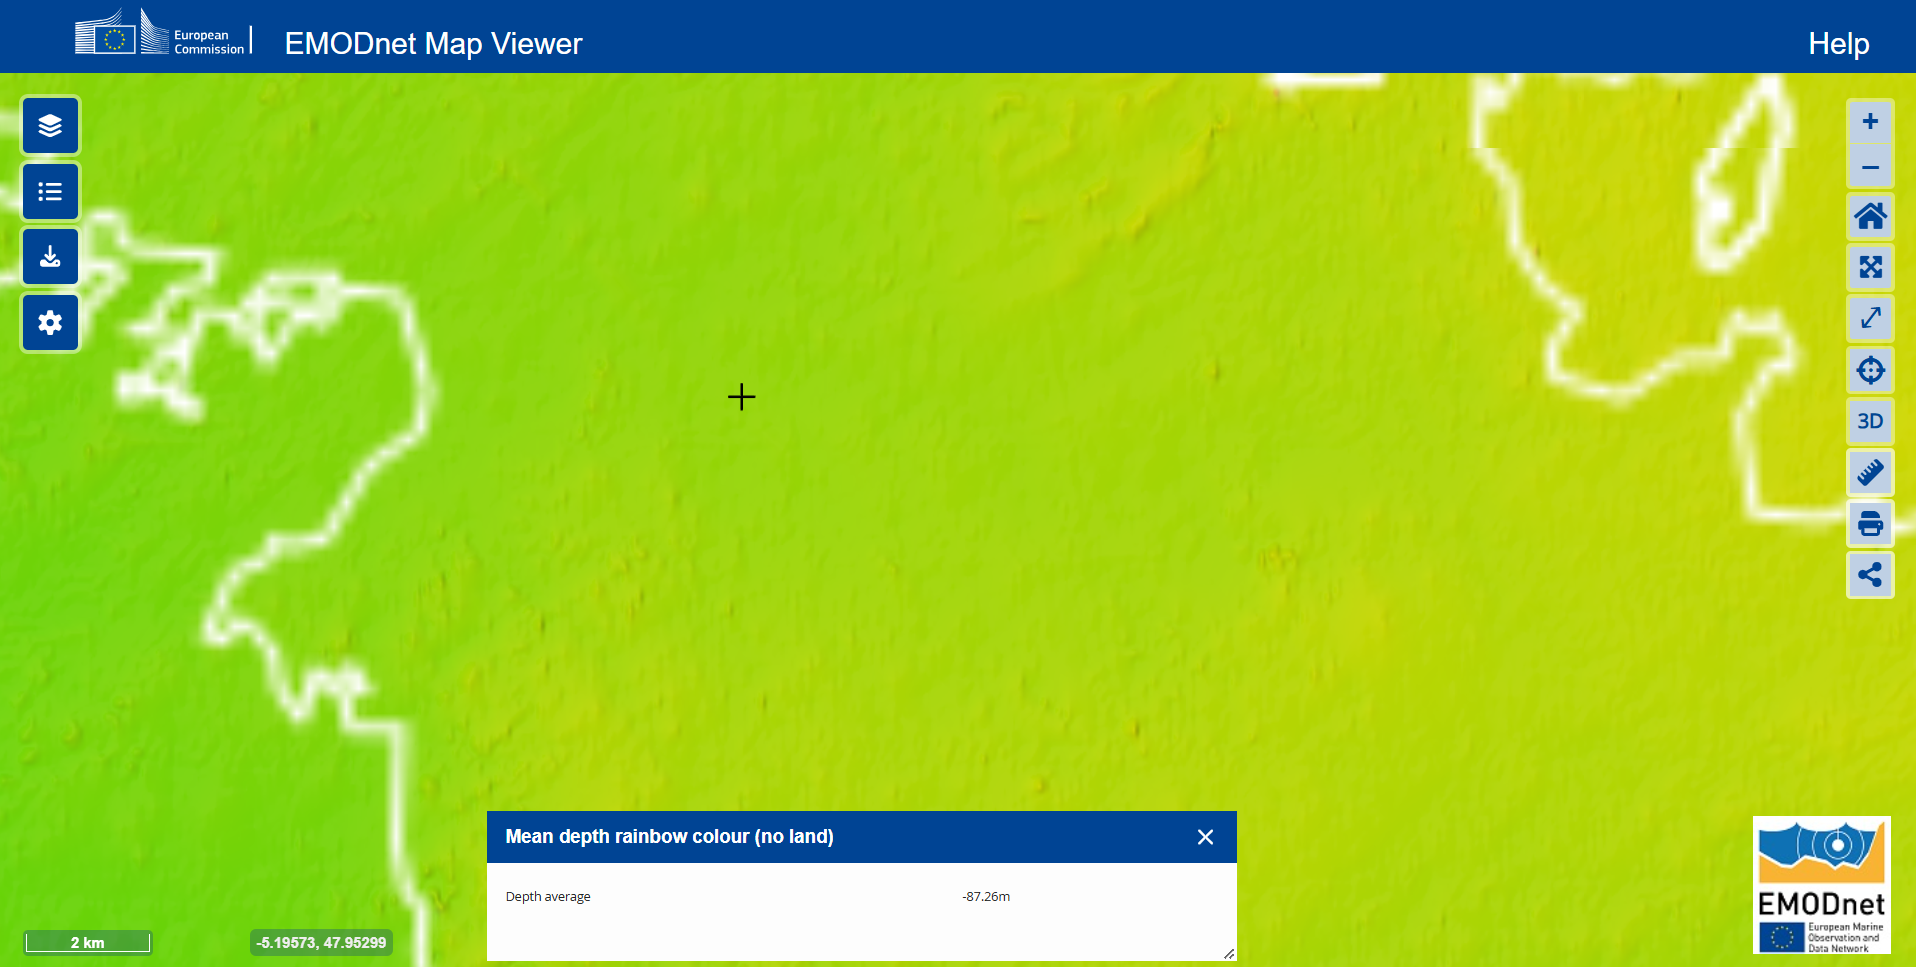
\includegraphics[width=\linewidth]{figures/emodnet_depth.png}
  \caption{EMODnet bathymetry viewer near the site.}
\end{subfigure}
\caption{Site selection data.}
\label{fig:site}
\end{figure}

%====================================================================
\section{Data and methods}
%====================================================================

\paragraph{Wave data.}
I used the Copernicus Marine global wave reanalysis (Météo-France MFWAM spectral model forced by ERA5 winds, \SI{0.2}{\degree} resolution) \cite{cmems}.
A $3\times2$ grid-point box around the site was downloaded with three variables: the spectral significant wave height $\Hs$ (\texttt{VHM0}), the mean period $\Tm$ (\texttt{VTM02}) and the mean direction the waves come from, $\theta_m$ (\texttt{VMDR}).
All analyses use the single grid point closest to the site (\SI{48.0}{\degree N}, \SI{5.4}{\degree W}).
Across the six grid points of the box, the mean $\Hs$ varies by less than \SI{0.2}{m}, so the results are not sensitive to this choice.
No buoy observations were available at this site to validate the model.

\paragraph{Mean and seasonal analysis.}
I computed the averages of $\Hs$ and $\Tm$ over the whole record.
Directions are angles, so their average is the circular mean $\bar\theta=\operatorname{atan2}(\overline{\sin\theta},\overline{\cos\theta})$.
The circular spreading is $\sigma_\theta=\sqrt{-2\ln R}$, where $R$ is the mean resultant length.
To look for trends, I computed annual means and tested them with a least-squares fit and with a non-parametric Mann--Kendall test (Theil--Sen slope).
The monthly climatology is the mean over all years for each calendar month.

\paragraph{Wave regimes.}
The deep-water wavelength is $L_0=gT^2/2\pi$.
Following linear wave theory, a wave is in deep water when $h>L_0/2$ (i.e.\ $T<\sqrt{4\pi h/g}$) and in shallow water when $h<L_0/20$.
Wave non-linearity is measured by the steepness $\Hs/L_0$:
\begin{itemize}
  \item Waves are treated as \emph{linear} when $\Hs/L_0<0.02$. Below this value, the second-order Stokes correction to the crest height, $ka/2=\pi H/(2L)$, is below \SI{3}{\percent}.
  \item Waves become \emph{weakly non-linear (Stokes)} as the steepness increases.
  \item Waves reach the breaking limit at $H/L\approx1/7$.
\end{itemize}
The Ursell number $U_r=HL^2/h^3$ is used to check whether the cnoidal (shallow-water) regime is relevant.

All figures and numbers in this report come from one script (\texttt{analysis.py}, provided with the report).

%====================================================================
\section{Results}
%====================================================================

\subsection{Question 1 -- Mean wave conditions and long-term trends}\label{sec:q1}

\begin{figure}[H]
\centering
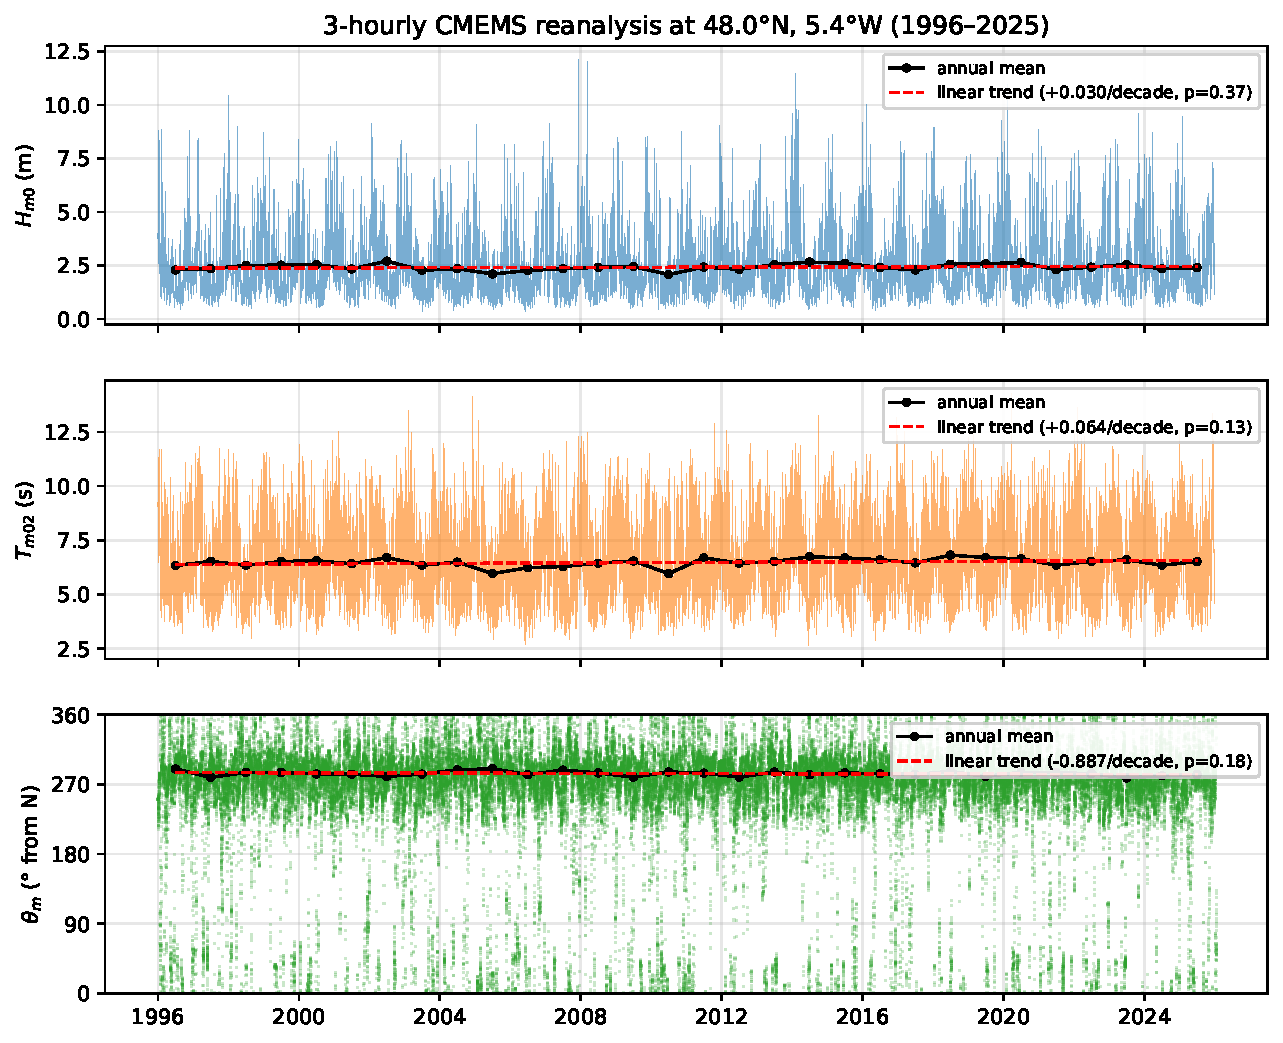
\includegraphics[width=0.8\linewidth]{figures/wave_timeseries.pdf}
\caption{Time series of $\Hs$, $\Tm$ and $\theta_m$ (3-hourly), with annual means (black) and linear trends of the annual means (red, slope and $p$-value in the legend).}
\label{fig:ts}
\end{figure}

\begin{table}[H]
\centering\small
\caption{Long-term statistics (1996--2025) and trends of the annual means. Trends are given per decade; $p$-values are from the least-squares fit and the Mann--Kendall test.}
\label{tab:mean}
\resizebox{\linewidth}{!}{%
\begin{tabular}{lccccc}
\toprule
 & Mean & Std / spread & Range of annual means & Trend /decade & $p$ (LS / MK) \\
\midrule
$\Hs$ (m) & 2.42 & 1.40 & 2.07 (2010) -- 2.70 (2002) & $+0.03$ & 0.37 / 0.34 \\
$\Hs$ annual 99\textsuperscript{th} pct.\ (m) & 6.92 & -- & 5.92 (2010) -- 8.70 (2014) & $+0.02$ & 0.85 / 0.86 \\
$\Tm$ (s) & 6.48 & 1.67 & 5.96 (2010) -- 6.82 (2018) & $+0.06$ & 0.13 / 0.13 \\
$\theta_m$ (\si{\degree} from N) & 283.8 & 38.3 (circ.) & 278.4 (2023) -- 290.1 (2005) & $-0.9$ & 0.18 / 0.21 \\
\bottomrule
\end{tabular}}
\end{table}

The mean sea state at the site is $\overline{\Hs}=\SI{2.42}{m}$ (median \SI{2.04}{m}), $\overline{\Tm}=\SI{6.48}{s}$ and $\bar\theta_m=\SI{283.8}{\degree}$, i.e.\ waves come from the WNW (Table~\ref{tab:mean}).
The largest sea state in the record is $\Hs=\SI{12.16}{m}$, on 9 December 2007.
The time series (Fig.~\ref{fig:ts}) is dominated by the annual cycle, with large winter storm peaks above \SI{8}{m} almost every year.
Directions are concentrated between \SIrange{250}{320}{\degree}. Rare easterly events (\SI{4.5}{\percent} of the time) correspond to offshore winds blowing from land.

\question{Do any trends in the wave height, period, or direction exist over the time period? Do you expect there to be changes in the mean conditions during the 30-year lifetime of the wind turbine? If so, why?}

\textbf{No statistically significant trend is detected.}
The fitted slopes are very small: $+\SI{0.03}{m}$/decade for $\Hs$ (\SI{1}{\percent} of the mean per decade), $+\SI{0.06}{s}$/decade for $\Tm$ and $-\SI{0.9}{\degree}$/decade for the direction.
All $p$-values are larger than 0.1 with both tests, and the storm statistic (annual 99\textsuperscript{th} percentile of $\Hs$) shows no trend either.
These slopes are much smaller than the year-to-year variability.
For example, the mean winter (DJFM) $\Hs$ varies from \SI{2.60}{m} (2011) to \SI{4.34}{m} (2014), a coefficient of variation of \SI{12}{\percent}.
The 2013/14 winter was the most energetic in the record, consistent with the exceptional sequence of Atlantic storms observed along the European coast that winter \cite{masselink2016}.
Low-energy years such as 2010 correspond to strongly negative North Atlantic Oscillation (NAO) winters.
This variability is controlled by large-scale atmospheric patterns (NAO, West Europe Pressure Anomaly) \cite{castelle2017}.
Thirty years of data are therefore too short to separate a possible long-term trend from this natural variability.

\textbf{Over the 30-year lifetime of the turbine}, I do not expect large changes in the \emph{mean} conditions, but significant year-to-year variations must be expected:
\begin{enumerate}
  \item \textbf{Natural variability.} Several stormy or calm winters in a row can change the decadal mean $\Hs$ by about \SI{10}{\percent}. This matters for fatigue loads and for weather windows during installation and maintenance.
  \item \textbf{Climate change.} Global wave projections for the North-East Atlantic give small changes in mean $\Hs$ by the end of the century (a few percent, mostly a slight decrease), with low agreement between models \cite{morim2019}. Changes in the position of the storm tracks could modify storm intensity and direction more than the mean, so extremes are more uncertain than mean conditions.
  \item \textbf{Water level.} Sea-level rise (a few tens of cm over 30 years) is negligible compared with \SI{68}{m} depth, so it will not change the wave regime at the site.
\end{enumerate}
A stationary wave climate is therefore a reasonable assumption for design, as long as margins are added to cover interannual variability and uncertainty in the extremes.

\subsection{Question 2 -- Most common wave conditions}\label{sec:q2}

\begin{figure}[H]
\centering
\begin{minipage}[c]{0.60\linewidth}
  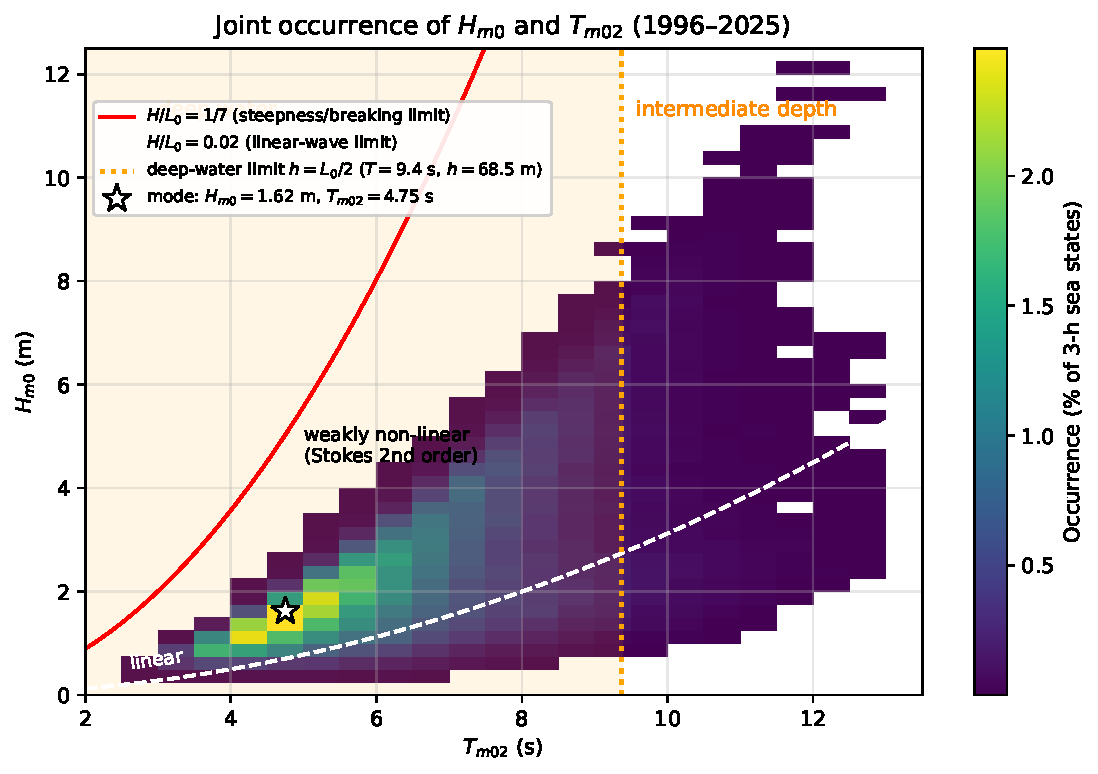
\includegraphics[width=\linewidth]{figures/wave_histogram.pdf}
\end{minipage}\hfill
\begin{minipage}[c]{0.38\linewidth}
  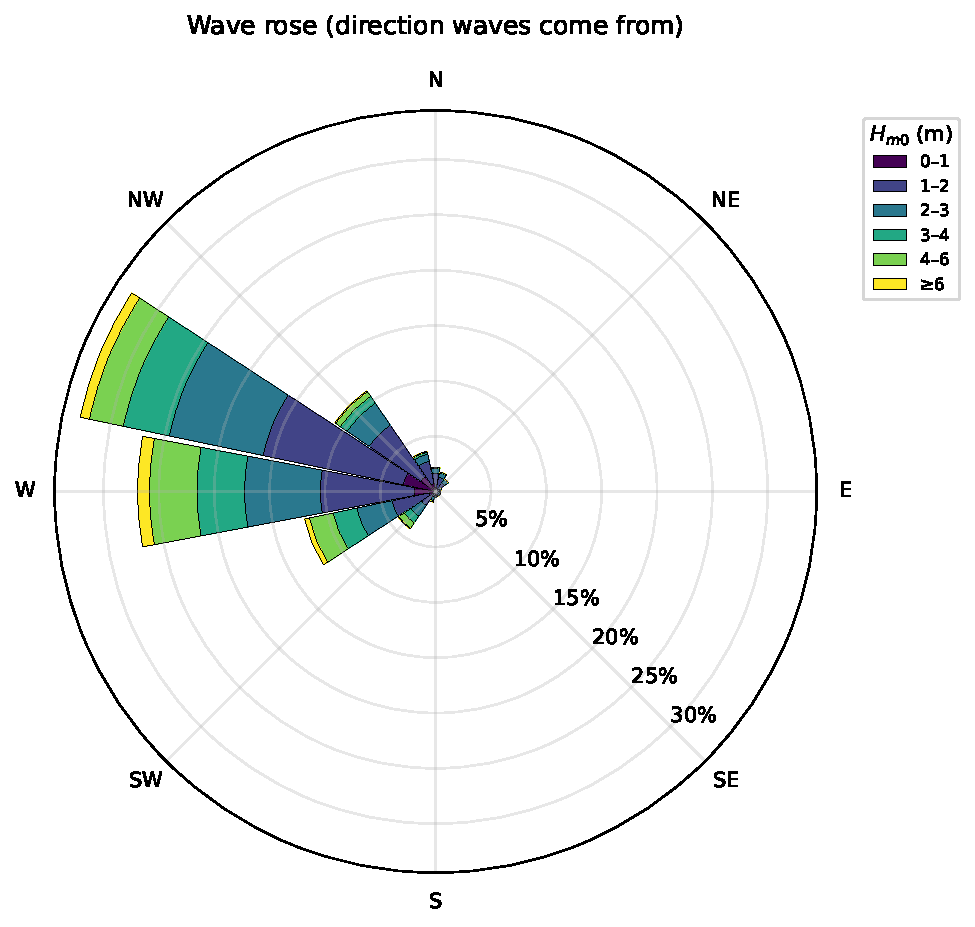
\includegraphics[width=\linewidth]{figures/wave_rose.pdf}
\end{minipage}
\caption{Left: joint occurrence of $\Hs$ and $\Tm$ (bins of \SI{0.25}{m}$\times$\SI{0.5}{s}), with the deep-water limit for $h=\SI{68.5}{m}$ (orange; deep water is the shaded side), the linear-wave limit $\Hs/L_0=0.02$ (white dashed) and the breaking steepness $1/7$ (red). Right: wave rose (direction waves come from) coloured by $\Hs$.}
\label{fig:hist}
\end{figure}

The most frequent sea state is $\Hs=\SI{1.62}{m}$, $\Tm=\SI{4.75}{s}$ (\num{2184} records, \SI{2.5}{\percent} of the time; Fig.~\ref{fig:hist}).
More broadly, \SI{36}{\percent} of the sea states have $\Hs$ between \SIrange{1}{3}{m} and $\Tm$ between \SIrange{5}{7}{s}.
The joint distribution follows a clear steepness relation: high waves are always associated with long periods ($\Tm>\SI{9}{s}$ for $\Hs>\SI{8}{m}$).

The wave rose shows a single dominant direction.
The four main sectors are WNW (\SI{33}{\percent}), W (\SI{27}{\percent}), WSW (\SI{12}{\percent}) and NW (\SI{11}{\percent}).
In total, \SI{82}{\percent} of the waves come from the \SIrange{225}{315}{\degree} sector, and almost all ($\SI{99}{\percent}$) of the sea states with $\Hs\geq\SI{6}{m}$ come from this sector.
This is the open Atlantic fetch: swells generated by North Atlantic depressions propagate freely towards Brittany.
Northerly and easterly directions are sheltered by the land (Brittany, Cornwall) and by short fetches.

\question{What is the water depth at this location? Indicate on the histogram for what wave conditions the waves are considered deep water waves? Linear waves?}

\textbf{Depth.} The mean water depth at the site is $h=\SI{68.5}{m}$ (EMODnet).

\textbf{Deep water} ($h>L_0/2$) corresponds to $T<\sqrt{4\pi h/g}=\SI{9.4}{s}$ (orange shaded area in Fig.~\ref{fig:hist}).
\begin{itemize}
  \item Using $\Tm$, \SI{95}{\percent} of the sea states are deep-water waves.
  \item The remaining long-period swells and storm waves are in \emph{intermediate depth} and feel the seabed.
  \item The energetic part of the spectrum is better represented by the peak period $T_p$, which is about $1.28\,\Tm$ for a JONSWAP spectrum. Using $T_p$, only about \SI{70}{\percent} of the sea states are in deep water.
  \item Shallow-water conditions ($h<L_0/20$, i.e.\ $T>\SI{30}{s}$) never occur at the site.
\end{itemize}

\textbf{Linear waves.} The region below the white dashed line ($\Hs/L_0<0.02$) contains \SI{12}{\percent} of the sea states: mainly long, low swells.
The remaining \SI{88}{\percent} have a steepness between 0.02 and $1/7$ (median 0.038). These are \emph{weakly non-linear} waves in the Stokes (second-order) range.
No sea state reaches the breaking steepness $1/7$.
Because the site is deep, non-linearity is controlled by the steepness rather than by the depth:
\begin{itemize}
  \item $\Hs/h\leq0.18$ even for the largest storm.
  \item The Ursell number stays small ($U_r\leq1.7\ll26$), so cnoidal or shallow-water theories are not needed.
\end{itemize}
Linear (Airy) theory is therefore a reasonable first approximation for most conditions. Second-order Stokes corrections should be considered for the steep storm waves used to compute the loads on the structure.

\subsection{Question 3 -- Seasonal variability}\label{sec:q3}

\begin{figure}[H]
\centering
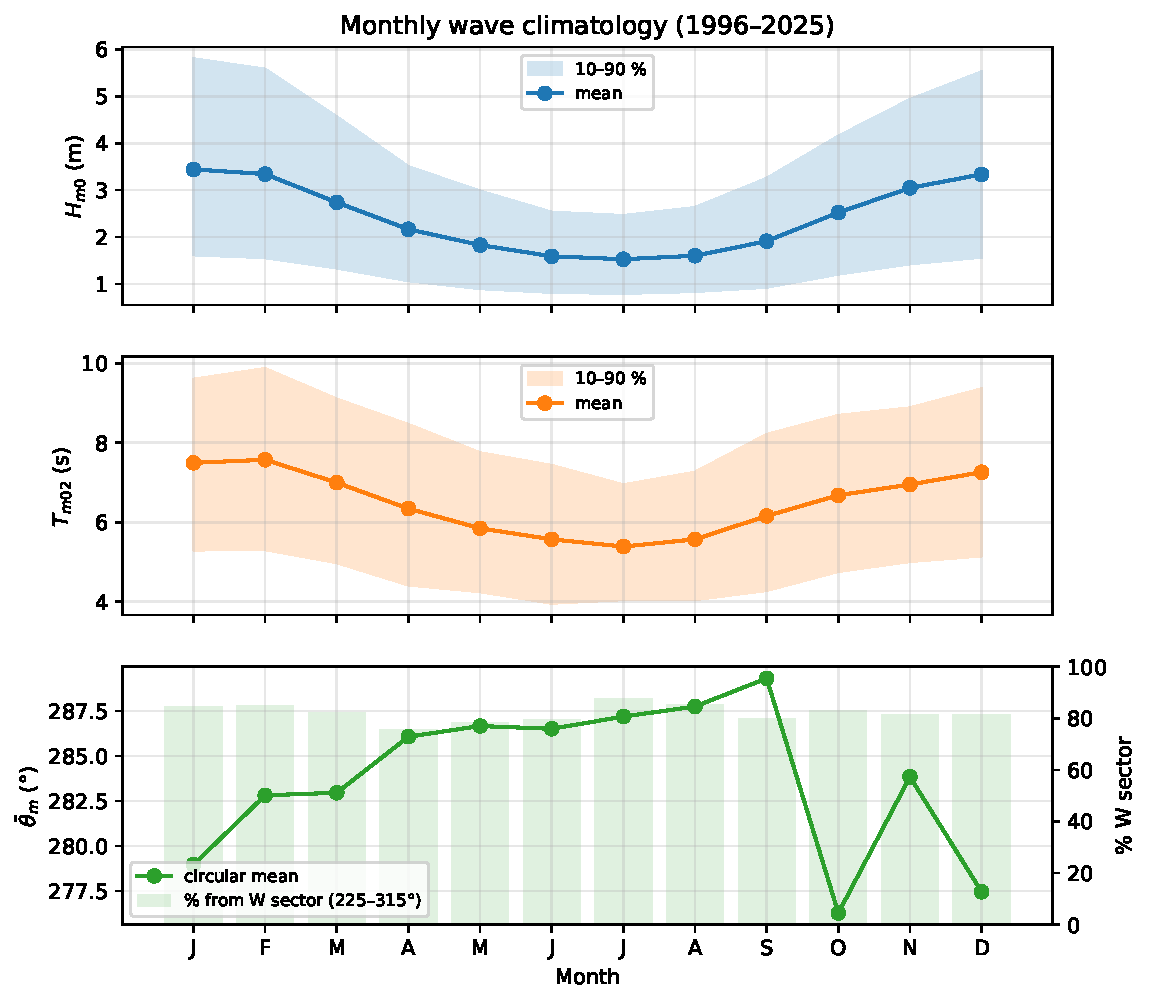
\includegraphics[width=0.66\linewidth]{figures/wave_monthly_climatology.pdf}
\caption{Monthly climatology of $\Hs$ and $\Tm$ (mean and 10--90\,\% range) and circular mean direction (line), with the percentage of waves from the W sector, \SIrange{225}{315}{\degree} (bars).}
\label{fig:month}
\end{figure}

\begin{table}[H]
\centering\small
\caption{Winter (DJF) versus summer (JJA) wave conditions.}
\label{tab:season}
\begin{tabular}{lcccc}
\toprule
 & $\overline{\Hs}$ (m) & $\overline{\Tm}$ (s) & $\bar\theta_m$ (\si{\degree}) & Time with $\Hs>\SI{4}{m}$ \\
\midrule
Winter (DJF) & 3.37 & 7.44 & 280 & \SI{31}{\percent} \\
Summer (JJA) & 1.57 & 5.51 & 287 & \SI{1.1}{\percent} \\
\bottomrule
\end{tabular}
\end{table}

\question{Do you observe any seasonal trends in wave height, period, or direction? If so, why?}

\textbf{Yes, there is a strong seasonal cycle in wave height and period, and a weak one in direction} (Fig.~\ref{fig:month}, Table~\ref{tab:season}).
\begin{itemize}
  \item \textbf{Wave height.} The mean $\Hs$ peaks in January (\SI{3.44}{m}) and is lowest in July (\SI{1.53}{m}), so winter waves are about twice as high as summer waves (four times more energetic, since energy scales with $H^2$). The spread also changes with the season: the 90\textsuperscript{th} percentile reaches \SI{5.8}{m} in January but only \SI{2.5}{m} in July. Seas with $\Hs>\SI{4}{m}$ occur \SI{31}{\percent} of the time in winter and almost never in summer.
  \item \textbf{Period.} $\Tm$ follows the same cycle, from \SI{7.6}{s} in February to \SI{5.4}{s} in July. Winter seas are dominated by long swells, while summer seas include more short, locally generated wind waves.
  \item \textbf{Direction.} Waves come from the W--WNW all year (\SIrange{80}{88}{\percent} from the W sector). The mean direction is slightly more westerly in winter (\SIrange{276}{283}{\degree}) than in late spring to September (\SIrange{286}{289}{\degree}).
\end{itemize}
\textbf{Why.} The cycle follows the seasonal behaviour of the North Atlantic storm track.
In winter, the strong equator--pole temperature gradient produces frequent, deep low-pressure systems. Their strong SW--W winds blow over very long fetches and durations, which generates high, long-period waves and swell travelling towards Brittany.
In summer, the Azores high extends north, the storm track moves towards higher latitudes and becomes weaker, and winds are lighter and more often from the NW--N (e.g.\ sea-breeze or Azores-high flow). As a result, waves are smaller and shorter, with a slightly more north-westerly direction.
The higher winter variability (wider 10--90\,\% range) reflects the alternation between storms and calmer periods.
For the project, operation and maintenance should be planned for April--September, and survival loads are governed by winter storms.

%====================================================================
\section{Discussion}
%====================================================================

\paragraph{Limitations and uncertainties.}
\begin{enumerate}
  \item \textbf{Model data.} The data are model results (MFWAM reanalysis) at \SI{0.2}{\degree} resolution, about \SI{8}{km} from the site, without validation against local measurements. Spectral wave models tend to underestimate the peaks of the largest storms. A comparison with nearby buoys (e.g.\ the CANDHIS network or the Brittany offshore buoys) or with the higher-resolution regional reanalyses (NWSHELF, ResourceCode) is recommended.
  \item \textbf{Water depth.} Depths from \SI{68}{m} to \SI{87}{m} were found within a few km. This changes the deep-water limit ($T<\SIrange{9.4}{10.6}{s}$) but not the conclusions.
\end{enumerate}

\paragraph{Next steps.}
\begin{itemize}
  \item Download the peak period $T_p$, which better describes the energetic part of the spectrum than $\Tm$.
  \item Add the wind and current roses (ERA5, CMEMS physics).
  \item Estimate the extreme wave conditions (Part I.B).
  \item Use the typical sea state identified here ($\Hs\approx\SI{1.6}{m}$, $\Tm\approx\SI{5}{s}$, from \SI{285}{\degree}) as an operational offshore boundary condition for the wave propagation model (Part II).
\end{itemize}

%====================================================================
\section{Conclusion}
%====================================================================

\begin{itemize}
  \item \textbf{Mean conditions.} The site (\SI{68.5}{m} deep, \SI{9}{m/s} mean wind) is exposed to the open Atlantic. The mean sea state is $\Hs=\SI{2.4}{m}$, $\Tm=\SI{6.5}{s}$ from the WNW.
  \item \textbf{Trends.} No significant trend is found over 1996--2025. Interannual variability (about $\pm$\SI{12}{\percent} in winter $\Hs$) dominates.
  \item \textbf{Most common conditions.} The typical sea state is $\Hs\approx\SI{1.6}{m}$, $\Tm\approx\SI{4.75}{s}$. Waves come mainly from the W--WNW and are mostly deep-water, weakly non-linear waves for which linear theory is a reasonable first approximation.
  \item \textbf{Seasonality.} Strong seasonality: winter waves are twice as high and \SI{2}{s} longer than summer waves.
\end{itemize}

%====================================================================
\begin{thebibliography}{99}\small
\bibitem{cmems} E.U. Copernicus Marine Service Information (CMEMS). \emph{Global Ocean Waves Reanalysis}, product GLOBAL\_MULTIYEAR\_WAV\_001\_032. \url{https://doi.org/10.48670/moi-00022}.
\bibitem{windeurope2017} WindEurope (2017). \emph{Floating offshore wind vision statement}.
\bibitem{masselink2016} G. Masselink et al. (2016). Extreme wave activity during 2013/2014 winter and morphological impacts along the Atlantic coast of Europe. \emph{Geophys. Res. Lett.}, 43, 2135--2143.
\bibitem{castelle2017} B. Castelle et al. (2017). A new climate index controlling winter wave activity along the Atlantic coast of Europe: the West Europe Pressure Anomaly. \emph{Geophys. Res. Lett.}, 44, 1384--1392.
\bibitem{morim2019} J. Morim et al. (2019). Robustness and uncertainties in global multivariate wind-wave climate projections. \emph{Nature Climate Change}, 9, 711--718.
\end{thebibliography}

\end{document}
